% Paste this first block over the Benchmark Performance Overview table.
\begin{table}[!htbp]
\centering
\footnotesize
\setlength{\tabcolsep}{2.5pt}
\caption{Overall CSV-reported Macro-F1 across the three Phase 2 hybrid benchmarks. Foundation-model rows show all-language rehearsal; from-scratch baseline results are unchanged. WiLI-2018 has no Arabic class.}
\label{tab:sota_overall_summary}
\resizebox{\columnwidth}{!}{%
\begin{tabular}{lccc}
\toprule
\textbf{Model Family} & \textbf{FLORES+} & \textbf{CommonLID} & \textbf{WiLI-18} \\
\midrule
\multicolumn{4}{l}{\textit{\textbf{From-Scratch Baselines} (Trained on Uniform 110k)}} \\
Multinomial NB & 0.9332 & 0.9342 & 0.9785 \\
Linear SVM & 0.9342 & 0.8895 & 0.9679 \\
Char $n$-gram + LogReg & 0.9298 & 0.8907 & 0.9750 \\
fastText (from scratch) & 0.9281 & 0.8758 & 0.9584 \\
XGBoost & 0.9181 & 0.8734 & 0.9215 \\
Char-CNN (1D-CNN) & 0.9177 & 0.8398 & 0.8790 \\
Char-BiGRU (Recurrent) & 0.9111 & 0.8166 & 0.8770 \\
\midrule
\multicolumn{4}{l}{\textit{\textbf{Foundation Models: All-Language Rehearsal}}} \\
XLM-R Base & \textbf{0.9995} & 0.9723 & \textbf{0.9829} \\
ConLID & 0.9947 & 0.9643 & 0.9769 \\
fastText LID-176 & 0.9988 & \textbf{0.9771} & 0.9819 \\
GlotLID v3 & 0.9993 & 0.9736 & 0.9814 \\
NLLB LID-218 & 0.9994 & 0.9640 & 0.9811 \\
OpenLID-v3 & 0.9989 & 0.9654 & 0.9817 \\
\bottomrule
\end{tabular}%
}
\end{table}

% Paste this four-panel FLORES+ figure near the start of Phase 2.
\begin{figure*}[!t]
\centering
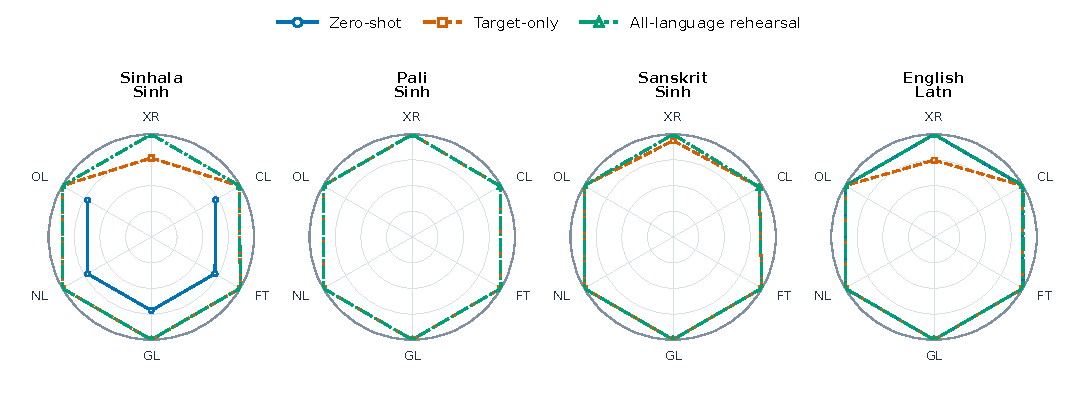
\includegraphics[width=\textwidth]{figures/radar_flores_four_languages_three_regimes.pdf}
\caption{FLORES+ per-language F1 for four representative languages across zero-shot, target-only fine-tuning, and all-language rehearsal. The 0--1 spokes clockwise from the top are XR (XLM-R Base), CL (ConLID), FT (fastText LID-176), GL (GlotLID v3), NL (NLLB LID-218), and OL (OpenLID-v3). An absent zero-shot profile for Pali or Sanskrit is N/A, not zero.}
\label{fig:radar_flores_four}
\end{figure*}

% Paste this combined block over the Detailed Hybrid Benchmark Results appendix tables.
\begin{table*}[p]
\centering
\scriptsize
\setlength{\tabcolsep}{1.4pt}
\renewcommand{\arraystretch}{0.78}
\caption{FLORES+ hybrid benchmark: per-language F1 and Macro-F1 across three training regimes.}
\label{tab:flores_full}
\begin{tabular}{l ccc cccccccc c}
\toprule
\textbf{Model} & \textbf{Sinh-Sinh} & \textbf{Pali-Sinh} & \textbf{San-Sinh} & \textbf{San-Deva} & \textbf{Eng-Latn} & \textbf{Tam-Taml} & \textbf{Hin-Deva} & \textbf{Ben-Beng} & \textbf{Ara-Arab} & \textbf{Fre-Latn} & \textbf{Ger-Latn} & \textbf{Macro F1} \\
\midrule
\multicolumn{13}{l}{\textit{Zero-shot results}} \\
XLM-R Base & -- & -- & -- & -- & 0.9985 & -- & 0.6836 & -- & 1.0000 & 0.9990 & 1.0000 & 0.4256 \\
ConLID & 0.7230 & -- & -- & 0.9985 & 0.9960 & 1.0000 & 0.9970 & 1.0000 & 0.6306 & 1.0000 & 0.9970 & 0.7584 \\
fastText LID-176 & 0.7152 & -- & -- & 0.9583 & 1.0000 & 1.0000 & 0.9624 & 1.0000 & 1.0000 & 1.0000 & 1.0000 & 0.7851 \\
GlotLID v3 & 0.7155 & -- & -- & 0.9945 & 1.0000 & 1.0000 & 0.9931 & 0.9995 & 0.9297 & 1.0000 & 1.0000 & 0.7848 \\
NLLB LID-218 & 0.7158 & -- & -- & 0.9890 & 0.9995 & 1.0000 & 0.9907 & 1.0000 & 0.9995 & 0.9995 & 0.9990 & 0.7903 \\
OpenLID-v3 & 0.7158 & -- & -- & 0.9885 & 0.9990 & 1.0000 & 0.9882 & 1.0000 & 1.0000 & 0.9975 & 0.9995 & 0.7899 \\
\midrule
\multicolumn{13}{l}{\textit{Target-only fine-tuning}} \\
XLM-R Base & 0.7696 & 0.9985 & 0.9381 & 0.0000 & 0.7483 & 0.0000 & 0.0000 & 0.0000 & 0.0000 & 0.9865 & 0.0059 & 0.4043 \\
ConLID & 0.9932 & 0.9904 & 0.9690 & 0.9985 & 0.9960 & 1.0000 & 0.9970 & 1.0000 & 0.6334 & 1.0000 & 0.9970 & 0.9613 \\
fastText LID-176 & 0.9988 & 0.9982 & 0.9966 & 0.9995 & 1.0000 & 1.0000 & 1.0000 & 1.0000 & 1.0000 & 1.0000 & 1.0000 & 0.9994 \\
GlotLID v3 & 0.9991 & 0.9990 & 0.9985 & 0.9950 & 1.0000 & 1.0000 & 0.9931 & 0.9995 & 0.9308 & 1.0000 & 1.0000 & 0.9923 \\
NLLB LID-218 & 0.9995 & 0.9994 & 0.9992 & 0.9905 & 1.0000 & 1.0000 & 0.9926 & 1.0000 & 1.0000 & 0.9995 & 1.0000 & 0.9983 \\
OpenLID-v3 & 0.9995 & 0.9994 & 1.0000 & 0.9895 & 0.9995 & 1.0000 & 0.9892 & 1.0000 & 1.0000 & 0.9970 & 0.9995 & 0.9976 \\
\midrule
\multicolumn{13}{l}{\textit{All-language rehearsal}} \\
XLM-R Base & 0.9996 & 0.9993 & 0.9996 & 0.9980 & 1.0000 & 0.9995 & 0.9980 & 1.0000 & 1.0000 & 1.0000 & 1.0000 & 0.9995 \\
ConLID & 0.9933 & 0.9907 & 0.9693 & 0.9985 & 0.9995 & 1.0000 & 0.9985 & 1.0000 & 0.9920 & 1.0000 & 1.0000 & 0.9947 \\
fastText LID-176 & 0.9988 & 0.9982 & 0.9966 & 0.9965 & 1.0000 & 1.0000 & 0.9970 & 1.0000 & 1.0000 & 1.0000 & 1.0000 & 0.9988 \\
GlotLID v3 & 0.9993 & 0.9992 & 0.9992 & 0.9990 & 1.0000 & 1.0000 & 0.9990 & 1.0000 & 0.9970 & 1.0000 & 1.0000 & 0.9993 \\
NLLB LID-218 & 0.9995 & 0.9994 & 0.9996 & 0.9975 & 1.0000 & 1.0000 & 0.9975 & 1.0000 & 1.0000 & 1.0000 & 1.0000 & 0.9994 \\
OpenLID-v3 & 0.9994 & 0.9992 & 1.0000 & 0.9945 & 1.0000 & 1.0000 & 0.9946 & 1.0000 & 1.0000 & 1.0000 & 1.0000 & 0.9989 \\
\bottomrule
\end{tabular}
\vspace{4pt}
\caption{CommonLID hybrid benchmark: per-language F1 and Macro-F1 across three training regimes.}
\label{tab:common_full}
\begin{tabular}{l ccc cccccccc c}
\toprule
\textbf{Model} & \textbf{Sinh-Sinh} & \textbf{Pali-Sinh} & \textbf{San-Sinh} & \textbf{San-Deva} & \textbf{Eng-Latn} & \textbf{Tam-Taml} & \textbf{Hin-Deva} & \textbf{Ben-Beng} & \textbf{Ara-Arab} & \textbf{Fre-Latn} & \textbf{Ger-Latn} & \textbf{Macro F1} \\
\midrule
\multicolumn{13}{l}{\textit{Zero-shot results}} \\
XLM-R Base & -- & -- & -- & -- & 0.9475 & -- & 0.8889 & -- & 0.9928 & 0.9484 & 0.9679 & 0.4314 \\
ConLID & 0.7230 & -- & -- & 0.9591 & 0.8502 & 0.9878 & 0.9447 & 0.9623 & 0.7669 & 0.8975 & 0.8955 & 0.7261 \\
fastText LID-176 & 0.7152 & -- & -- & 0.8797 & 0.9725 & 1.0000 & 0.9689 & 0.9827 & 0.9924 & 0.9505 & 0.9685 & 0.7664 \\
GlotLID v3 & 0.7155 & -- & -- & 0.9634 & 0.9257 & 0.9878 & 0.9717 & 0.9791 & 0.9632 & 0.9256 & 0.9218 & 0.7594 \\
NLLB LID-218 & 0.7158 & -- & -- & 0.9282 & 0.9248 & 0.9747 & 0.9641 & 0.9866 & 0.9925 & 0.9292 & 0.9411 & 0.7597 \\
OpenLID-v3 & 0.7158 & -- & -- & 0.9556 & 0.8573 & 0.9818 & 0.9367 & 0.9800 & 0.9949 & 0.8912 & 0.9025 & 0.7469 \\
\midrule
\multicolumn{13}{l}{\textit{Target-only fine-tuning}} \\
XLM-R Base & 0.2780 & 0.9230 & 0.7387 & 0.0000 & 0.5953 & 0.0000 & 0.0000 & 0.0000 & 0.0016 & 0.8087 & 0.0021 & 0.3043 \\
ConLID & 0.9932 & 0.9782 & 0.9690 & 0.9591 & 0.8497 & 0.9878 & 0.9447 & 0.9611 & 0.7670 & 0.8975 & 0.8954 & 0.9275 \\
fastText LID-176 & 0.9988 & 0.9982 & 0.9966 & 0.9368 & 0.9737 & 0.9938 & 0.9698 & 0.9833 & 0.9903 & 0.9558 & 0.9693 & 0.9788 \\
GlotLID v3 & 0.9991 & 0.9989 & 0.9985 & 0.9633 & 0.9269 & 0.9878 & 0.9677 & 0.9822 & 0.9641 & 0.9277 & 0.9198 & 0.9669 \\
NLLB LID-218 & 0.9994 & 0.9893 & 0.9989 & 0.9295 & 0.9068 & 0.9875 & 0.9610 & 0.9863 & 0.9921 & 0.9211 & 0.9412 & 0.9648 \\
OpenLID-v3 & 0.9991 & 0.9234 & 0.9977 & 0.9557 & 0.8627 & 0.9818 & 0.9328 & 0.9809 & 0.9953 & 0.8919 & 0.9090 & 0.9482 \\
\midrule
\multicolumn{13}{l}{\textit{All-language rehearsal}} \\
XLM-R Base & 0.9984 & 0.9992 & 0.9966 & 0.9407 & 0.9785 & 0.9205 & 0.9823 & 0.9892 & 0.9941 & 0.9386 & 0.9573 & 0.9723 \\
ConLID & 0.9933 & 0.9862 & 0.9693 & 0.9587 & 0.9118 & 0.9878 & 0.9756 & 0.9805 & 0.9861 & 0.9219 & 0.9364 & 0.9643 \\
fastText LID-176 & 0.9988 & 0.9982 & 0.9966 & 0.9366 & 0.9727 & 1.0000 & 0.9798 & 0.9838 & 0.9936 & 0.9252 & 0.9627 & 0.9771 \\
GlotLID v3 & 0.9993 & 0.9991 & 0.9992 & 0.9380 & 0.9605 & 0.9878 & 0.9699 & 0.9922 & 0.9928 & 0.9351 & 0.9357 & 0.9736 \\
NLLB LID-218 & 0.9995 & 0.9972 & 0.9996 & 0.9235 & 0.9505 & 0.9474 & 0.9586 & 0.9906 & 0.9951 & 0.9014 & 0.9404 & 0.9640 \\
OpenLID-v3 & 0.9994 & 0.9695 & 0.9985 & 0.9544 & 0.9531 & 0.9818 & 0.9420 & 0.9858 & 0.9966 & 0.8934 & 0.9447 & 0.9654 \\
\bottomrule
\end{tabular}
\vspace{4pt}
\caption{WiLI-2018 hybrid benchmark: per-language F1 and Macro-F1 across three training regimes.}
\label{tab:wili_full}
\begin{tabular}{l ccc cccccccc c}
\toprule
\textbf{Model} & \textbf{Sinh-Sinh} & \textbf{Pali-Sinh} & \textbf{San-Sinh} & \textbf{San-Deva} & \textbf{Eng-Latn} & \textbf{Tam-Taml} & \textbf{Hin-Deva} & \textbf{Ben-Beng} & \textbf{Ara-Arab} & \textbf{Fre-Latn} & \textbf{Ger-Latn} & \textbf{Macro F1} \\
\midrule
\multicolumn{13}{l}{\textit{Zero-shot results}} \\
XLM-R Base & -- & -- & -- & -- & 0.9471 & -- & 0.6644 & -- & -- & 0.9910 & 0.9879 & 0.3590 \\
ConLID & 0.7230 & -- & -- & 0.9960 & 0.9331 & 0.9939 & 0.9879 & 0.9362 & -- & 0.9838 & 0.9670 & 0.7521 \\
fastText LID-176 & 0.7152 & -- & -- & 0.9939 & 0.9346 & 0.9928 & 0.9879 & 0.9350 & -- & 0.9920 & 0.9889 & 0.7540 \\
GlotLID v3 & 0.7155 & -- & -- & 0.9950 & 0.9313 & 0.9939 & 0.9154 & 0.9396 & -- & 0.9900 & 0.9754 & 0.7456 \\
NLLB LID-218 & 0.7158 & -- & -- & 0.9939 & 0.9392 & 0.9928 & 0.9868 & 0.9350 & -- & 0.9920 & 0.9869 & 0.7542 \\
OpenLID-v3 & 0.7158 & -- & -- & 0.9940 & 0.9564 & 0.9939 & 0.9734 & 0.9373 & -- & 0.9722 & 0.9723 & 0.7515 \\
\midrule
\multicolumn{13}{l}{\textit{Target-only fine-tuning}} \\
XLM-R Base & 0.8846 & 0.9987 & 0.9809 & 0.0000 & 0.6080 & 0.0000 & 0.0000 & 0.0000 & -- & 0.9429 & 0.0040 & 0.4419 \\
ConLID & 0.9932 & 0.9896 & 0.9690 & 0.9960 & 0.9357 & 0.9939 & 0.9879 & 0.9350 & -- & 0.9838 & 0.9670 & 0.9751 \\
fastText LID-176 & 0.9988 & 0.9982 & 0.9966 & 0.9950 & 0.9328 & 0.9928 & 0.9879 & 0.9350 & -- & 0.9920 & 0.9889 & 0.9818 \\
GlotLID v3 & 0.9991 & 0.9990 & 0.9985 & 0.9950 & 0.9313 & 0.9939 & 0.9071 & 0.9396 & -- & 0.9889 & 0.9712 & 0.9724 \\
NLLB LID-218 & 0.9995 & 0.9994 & 0.9992 & 0.9929 & 0.9420 & 0.9928 & 0.9868 & 0.9350 & -- & 0.9920 & 0.9889 & 0.9829 \\
OpenLID-v3 & 0.9995 & 0.9987 & 1.0000 & 0.9960 & 0.9518 & 0.9939 & 0.9744 & 0.9396 & -- & 0.9701 & 0.9765 & 0.9800 \\
\midrule
\multicolumn{13}{l}{\textit{All-language rehearsal}} \\
XLM-R Base & 0.9996 & 0.9993 & 0.9996 & 0.9960 & 0.9311 & 0.9928 & 0.9889 & 0.9451 & -- & 0.9910 & 0.9859 & 0.9829 \\
ConLID & 0.9933 & 0.9906 & 0.9693 & 0.9960 & 0.9254 & 0.9939 & 0.9889 & 0.9362 & -- & 0.9900 & 0.9858 & 0.9769 \\
fastText LID-176 & 0.9988 & 0.9982 & 0.9966 & 0.9950 & 0.9337 & 0.9928 & 0.9879 & 0.9350 & -- & 0.9930 & 0.9879 & 0.9819 \\
GlotLID v3 & 0.9993 & 0.9992 & 0.9992 & 0.9950 & 0.9282 & 0.9939 & 0.9858 & 0.9384 & -- & 0.9890 & 0.9859 & 0.9814 \\
NLLB LID-218 & 0.9995 & 0.9994 & 0.9996 & 0.9930 & 0.9272 & 0.9939 & 0.9858 & 0.9373 & -- & 0.9910 & 0.9839 & 0.9811 \\
OpenLID-v3 & 0.9994 & 0.9991 & 1.0000 & 0.9950 & 0.9291 & 0.9939 & 0.9858 & 0.9384 & -- & 0.9900 & 0.9859 & 0.9817 \\
\bottomrule
\end{tabular}
\end{table*}

% Paste this figure immediately after the combined appendix table.
\clearpage
\begin{figure*}[p]
\centering
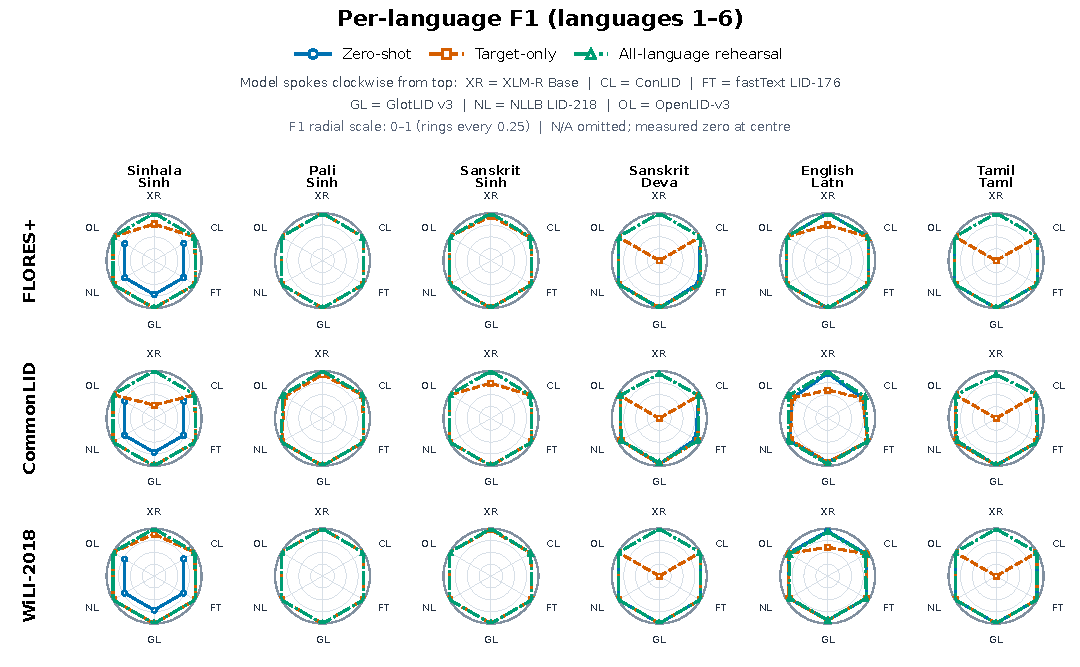
\includegraphics[width=0.96\textwidth]{figures/radar_grid_three_regimes_languages_1-6.pdf}
\par\vspace{-3pt}
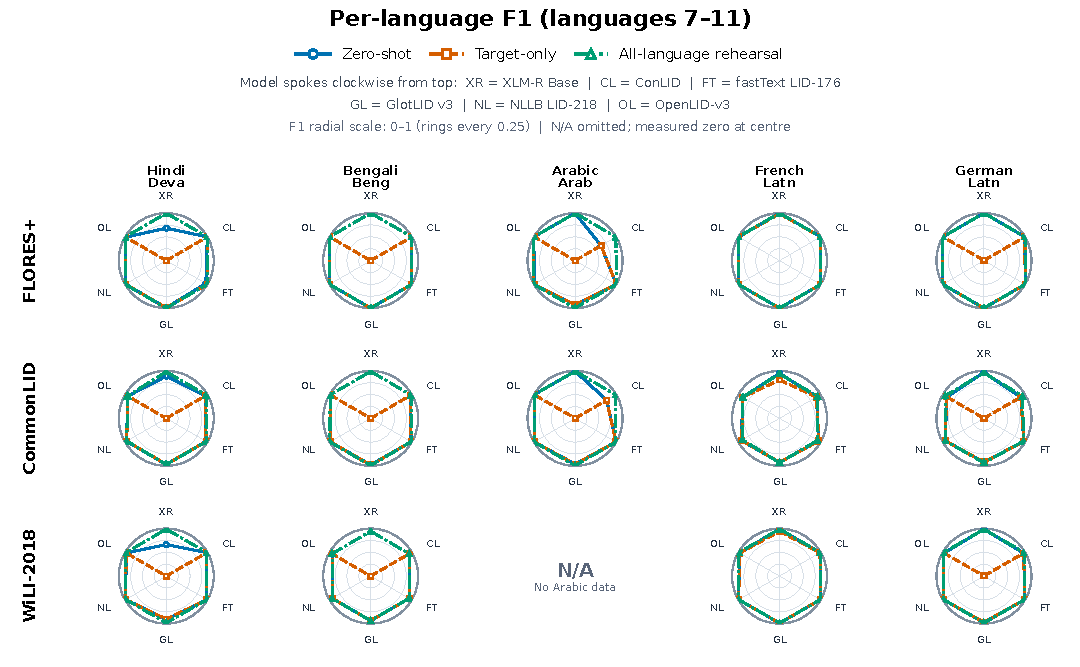
\includegraphics[width=0.96\textwidth]{figures/radar_grid_three_regimes_languages_7-11.pdf}
\caption{All 33 benchmark--language radar panels. The upper block contains languages 1--6 and the lower block languages 7--11; each block has FLORES+, CommonLID, and WiLI-2018 rows. Colored lines show zero-shot, target-only fine-tuning, and all-language rehearsal. WiLI-2018 Arabic is N/A.}
\label{fig:radar_all_33}
\end{figure*}
\clearpage
